% !TeX root = ./2020-21-COMP250-07-session-materials_screen.tex
% Adjust these for the path of the theme and its graphics, relative to this file
%\usepackage{beamerthemeFalmouthGamesAcademy}
\usepackage{../../beamerthemeFalmouthGamesAcademy}
\usepackage{multimedia}
\graphicspath{ {../../} }

% Default language for code listings
\lstset{language=C++,
        morekeywords={each,in,nullptr}
}

% For strikethrough effect
\usepackage[normalem]{ulem}
\usepackage{wasysym}

\usepackage{pdfpages}

% http://www.texample.net/tikz/examples/state-machine/
\usetikzlibrary{arrows,automata}

\newcommand{\modulecode}{COMP260}\newcommand{\moduletitle}{Distributed Systems}\newcommand{\sessionnumber}{5}

\begin{document}
\title{\sessionnumber: Procedural Content Generation}
\subtitle{\modulecode: \moduletitle}

\frame{\titlepage} 

\newcommand{\pictureslideb}[3]{
	\begin{frame}{#1}
		\begin{center}
			\includegraphics[height=0.6\textheight]{#2}
			
			\vspace{6pt}
			
			#3
		\end{center}
	\end{frame}
}

\newcommand{\pictureslide}[2]{
	\begin{frame}{#1}
		\begin{center}
			\includegraphics[height=0.6\textheight]{#2}
		\end{center}
	\end{frame}
}

\newcommand{\pictureslidew}[2]{
	\begin{frame}{#1}
		\begin{center}
			\includegraphics[width=\textwidth]{#2}
		\end{center}
	\end{frame}
}

\part{What is PCG?}
\frame{\partpage}

\begin{frame}{What is procedural content generation (PCG)?}
	\begin{itemize}
		\item<3-> \textbf{Procedural}: by computer program or algorithm,
			with little or no direct input from designer or user
		\item<2-> \textbf{Content}: levels, maps, art, animations, stories, items,
			quests, music, weapons, vehicles, characters, ...
		\item<1-> \textbf{Generation}: creating stuff
	\end{itemize}
\end{frame}

\begin{frame}{Types of PCG}
	\begin{itemize}
		\pause\item \textbf{Online}
			\begin{itemize}
				\pause\item Generate content at run-time
				\pause\item Part of the game
			\end{itemize}
		\pause\item \textbf{Offline}
			\begin{itemize}
				\pause\item Generate content at design-time
				\pause\item Tool for developers
			\end{itemize}
	\end{itemize}
\end{frame}

\begin{frame}{PCG $\neq$ randomness}
	\begin{itemize}
		\pause\item Many PCG systems use random numbers, but randomness in itself is not PCG
		\pause\item Can have PCG without randomness, e.g.\ based on fractals or simulations
		\pause\item Randomness in PCG is generally \textbf{constrained} to produce desired content
		\pause\item Shuffling a deck of cards for a game of Solitaire is \textbf{not} PCG!
	\end{itemize}
\end{frame}

% \begin{frame}{Not to be confused with...}
% 	\begin{itemize}
% 		\pause\item \textbf{Procedural Rhetoric} / \textbf{Procedurality} (Bogost)
% 		\pause\item ``the art of persuasion through rule-based representations and interactions,
% 			rather than the spoken word, writing, images, or moving pictures''
% 		\pause\item There: ``procedural'' = ``rule-based''
% 		\pause\item Here: ``procedural'' = ``algorithmic''
% 	\end{itemize}
% \end{frame}

\begin{frame}{Why PCG?}
	\begin{itemize}
		\pause\item More content for less development effort
		\pause\item Decrease development costs
		\pause\item Increase replayability
		\pause\item Decrease storage requirements
		\pause\item Allow game mechanics based on unseen content
	\end{itemize}
\end{frame}

\begin{frame}{Further reading}
	Noor Shaker, Julian Togelius and Mark J. Nelson.
	\textit{Procedural Content Generation in Games: A textbook and an overview of current research}.
	Springer, 2016.
	
	Available online: \url{http://pcgbook.com}
\end{frame}


\pictureslide{The Binding of Isaac (2011)}{isaac}
\pictureslide{Enter The Gungeon (2016)}{enterthegungeon}
\pictureslide{Spelunky (2008)}{spelunky}
\pictureslide{Dwarf Fortress (2006)}{dwarffortress}
\pictureslide{No Man's Sky (2016)}{nomanssky}


%\newcommand{\pictureslideb}[3]{
	\begin{frame}{#1}
		\begin{center}
			#3
			
			\vspace{6pt}
			
			\includegraphics[height=0.6\textheight]{#2}
		\end{center}
	\end{frame}
}

\newcommand{\pictureslide}[2]{
	\begin{frame}{#1}
		\begin{center}
			\includegraphics[height=0.6\textheight]{#2}
		\end{center}
	\end{frame}
}

\part{What was the first computer?}
\frame{\partpage}

\pictureslideb{Antikythera Mechanism ($\sim$150 BC)}{antikythera}{First mechanical computer?}
\pictureslideb{Babbage's Difference and Analytical Engines (1837)}{difference_engine}{First mechanical computer in modern age}
\pictureslideb{Colossus (1943)}{colossus}{First programmable electronic computer}
\pictureslideb{ENIAC (1946)}{eniac}{First general-purpose computer}
\pictureslideb{Manchester Small-Scale Experimental Machine (1948)}{manchester}{First stored program computer}
\pictureslideb{EDSAC (1949)}{edsac}{Many firsts in mathematics and science}
\pictureslideb{PDP-1 (1959)}{pdp1}{Influenced ``hacker culture''}
\pictureslideb{Datapoint 2200 (1970)}{datapoint2200}{First microcomputer}
\pictureslideb{Commodore VIC 20 (1980)}{vic20}{First computer to sell 1 million units}
\pictureslideb{IBM Personal Computer Model 5150 (1981)}{ibm_5150}{Precursor to the modern PC}

\part{What was the first computer game?}
\frame{\partpage}

\pictureslideb{Cathode Ray Tube Amusement Device (1948)}{crt}{First interactive electronic game}
\pictureslideb{Chess AI on the Ferranti Mark I (1951)}{ferranti}{First chess program}
\pictureslideb{Bertie the Brain (1950)}{bertie}{First computer game with a visual display}
\pictureslideb{OXO (1951)}{oxo}{First game with visuals on a general-purpose computer}
\pictureslideb{Tennis for Two (1959)}{tennis}{First to be created purely for entertainment}
\pictureslideb{SpaceWar! (1962)}{spacewar}{First widely available game, inspired first arcade games}
\pictureslideb{Pong (1972)}{pong}{First commercially successful game}

\part{What was the first games console?}
\frame{\partpage}

\pictureslideb{The Brown Box (1967)}{brownbox}{First prototype console}
\pictureslideb{Magnavox Odyssey (1972)}{magnavox}{First commercial console}

\begin{frame}{Game console timeline}
	\begin{center}
		\url{http://www.onlineeducation.net/videogame_timeline/video-game-timeline.jpg}
		
		(A little out of date!)
	\end{center}
\end{frame}


%% !TeX root = ./2020-21-COMP250-07-session-materials_screen.tex
\part{A selection of PCG techniques}
\frame{\partpage}

\pictureslideb{Combining hand-authored blocks}{spelunky_gen}{\url{http://tinysubversions.com/spelunkyGen2/}}

\begin{frame}{Perlin noise}
	\begin{columns}
		\begin{column}{0.4\textwidth}
			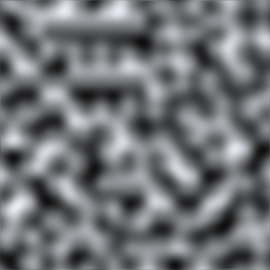
\includegraphics[width=\textwidth]{perlin}
		\end{column}
		\begin{column}{0.55\textwidth}
			\begin{itemize}
                \pause\item A ``smooth'' random number generator
                \pause\item Often used for terrain generation
                \pause\item 2D: use as height map
                \pause\item 3D: apply threshold to generate caves
			\end{itemize}
		\end{column}
	\end{columns}
\end{frame}

\begin{frame}{Fractals}
	\begin{columns}
		\begin{column}{0.4\textwidth}
			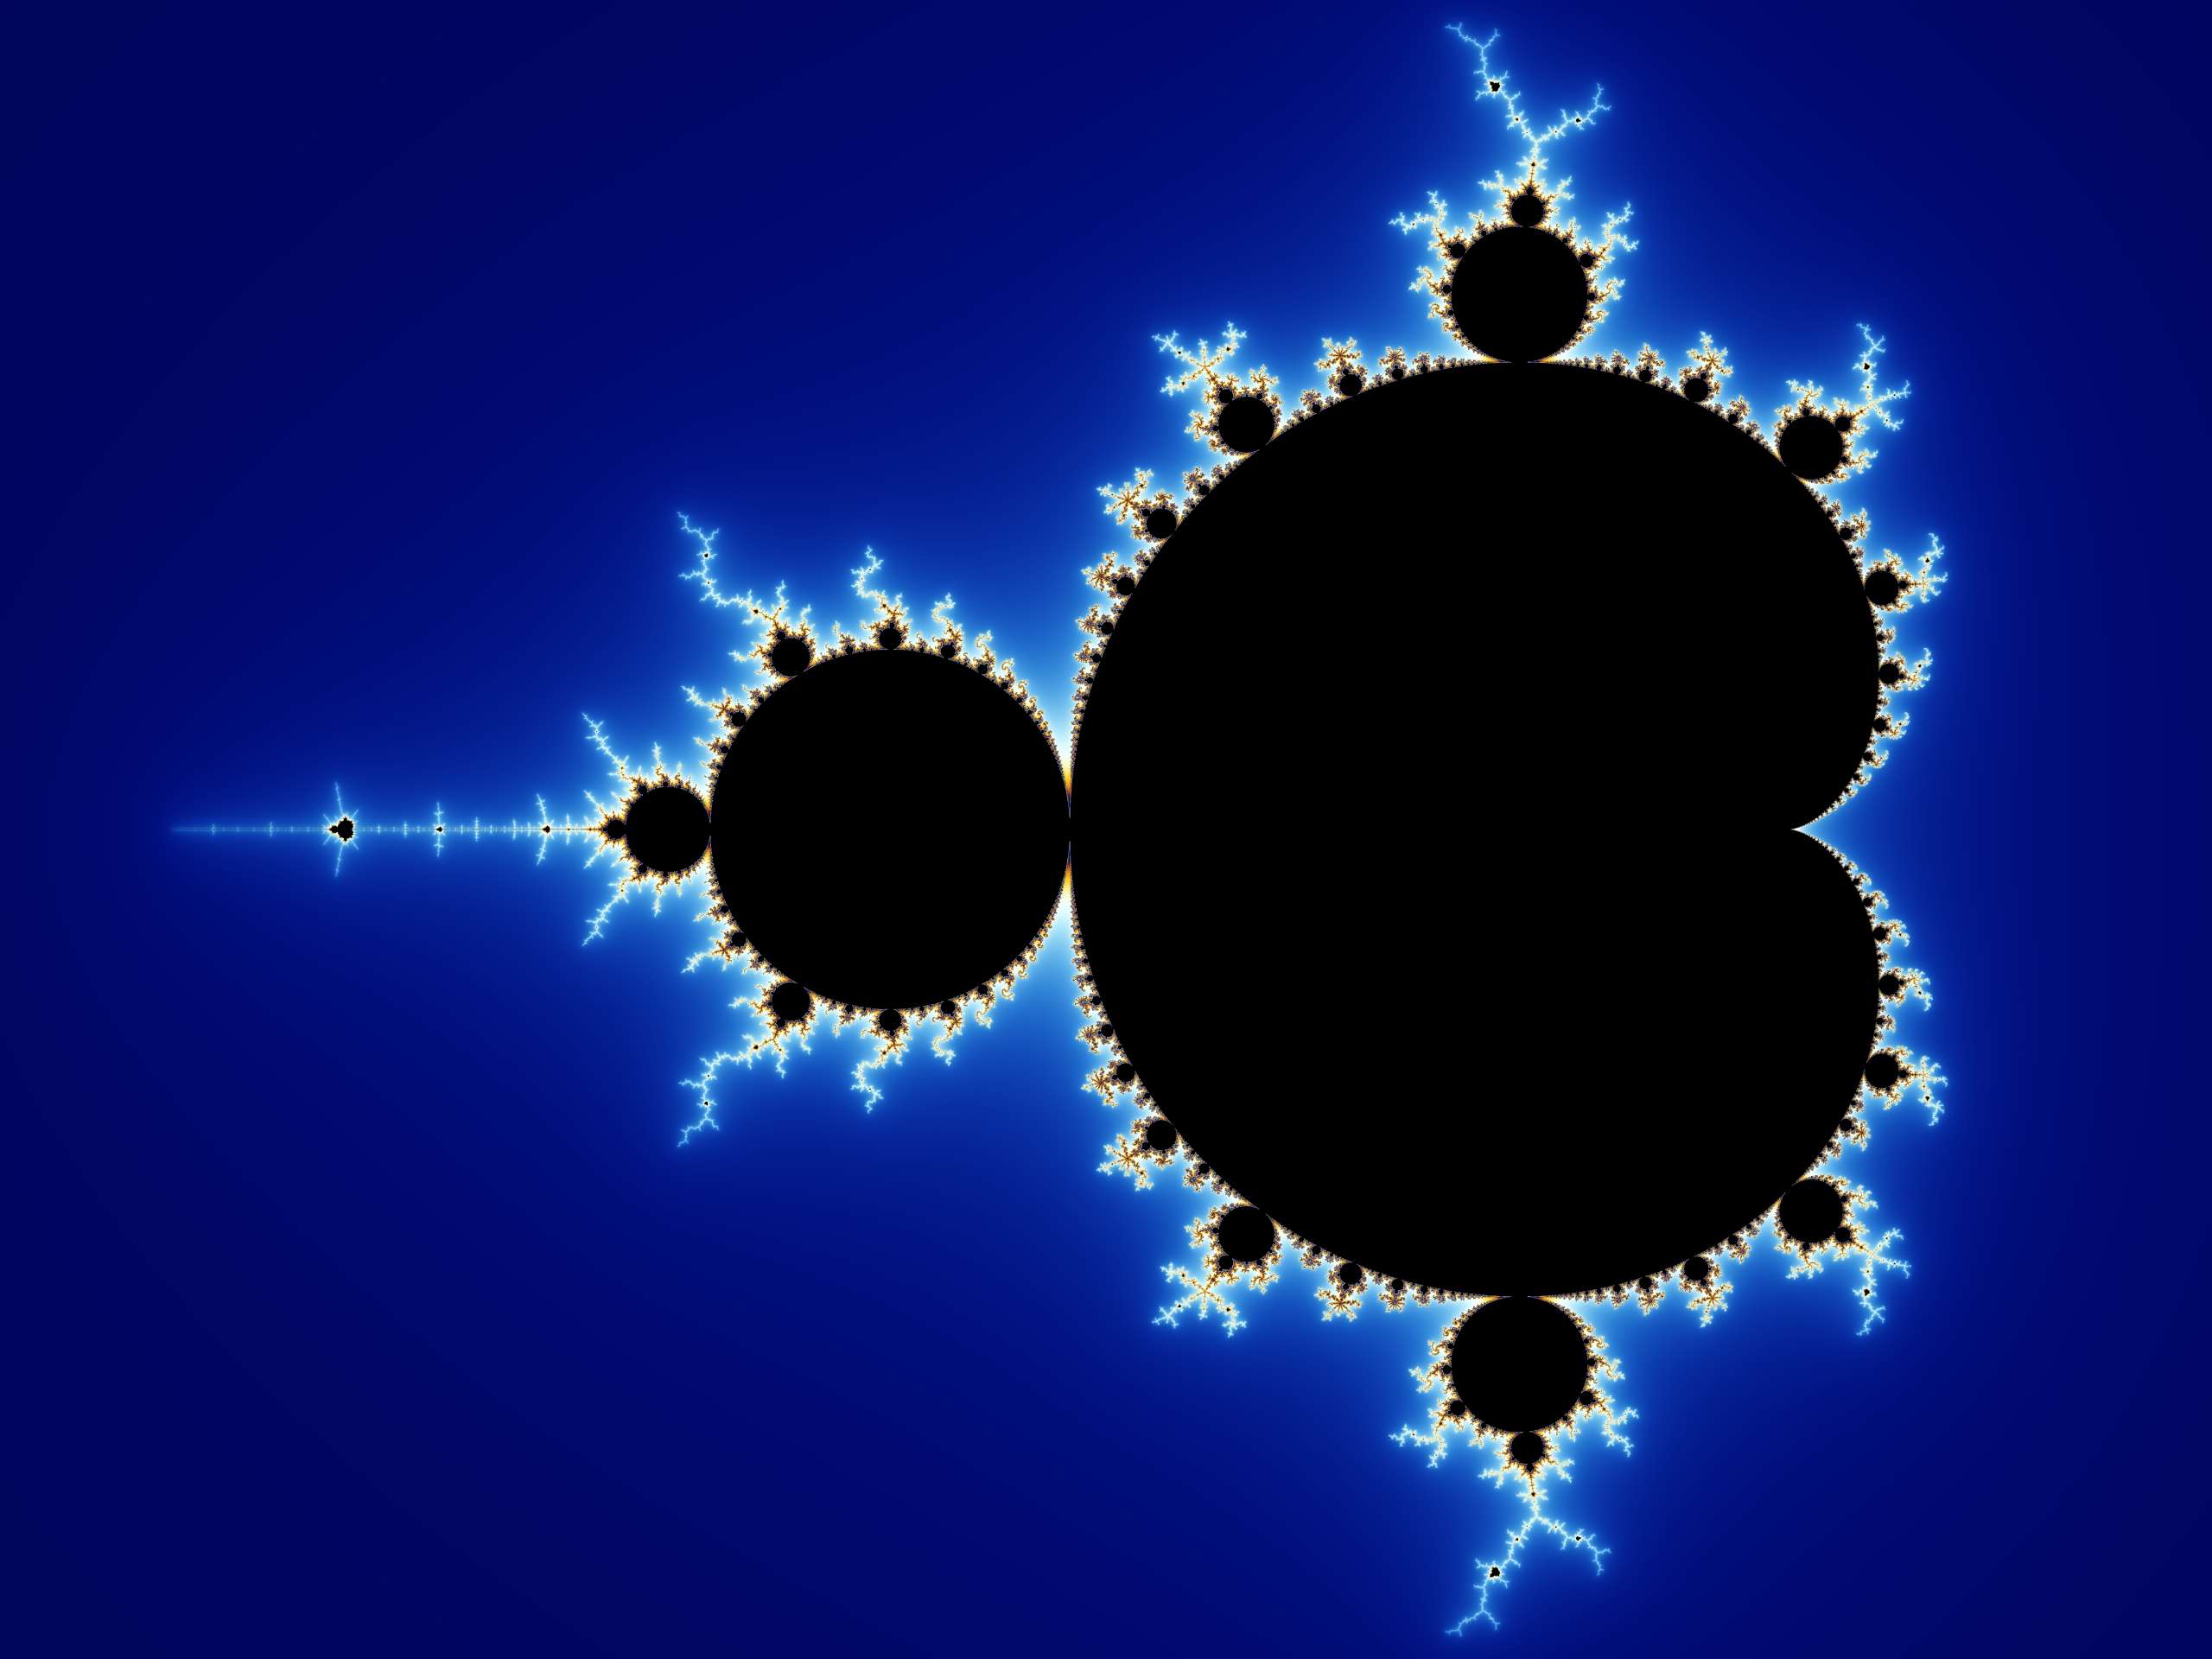
\includegraphics[width=\textwidth]{mandelbrot}
		\end{column}
		\begin{column}{0.55\textwidth}
			\begin{itemize}
                \pause\item Some simple mathematical formulae can give rise to complex emergent structures
                \pause\item E.g.\ the Mandelbrot set: generated by iteration of the formula 
                    $$ z_{i+1} = z_i^2 + c $$
			\end{itemize}
		\end{column}
	\end{columns}
\end{frame}

\begin{frame}{L-Systems}
	\begin{columns}
		\begin{column}{0.4\textwidth}
			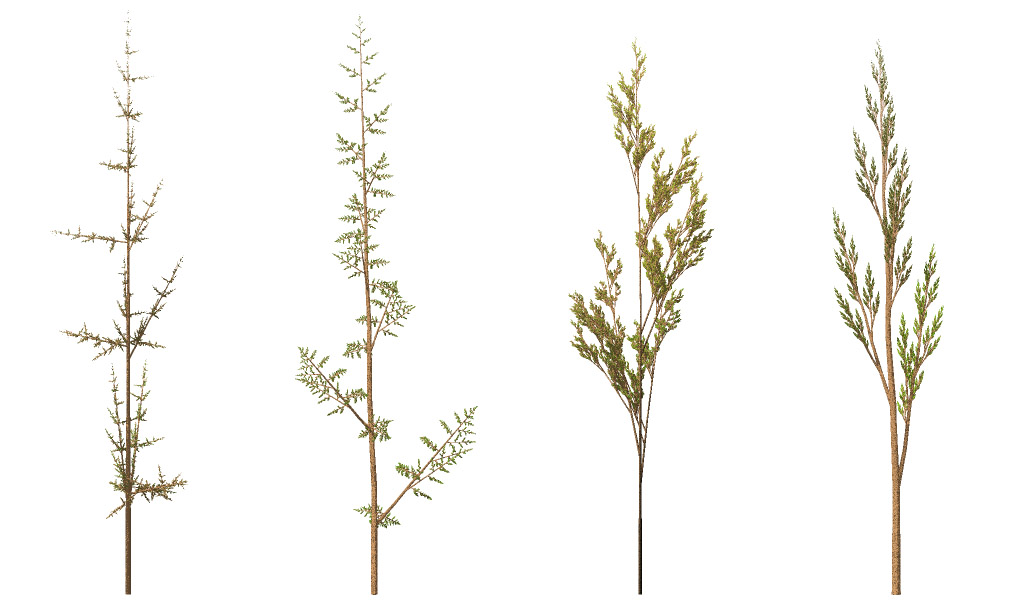
\includegraphics[width=\textwidth]{lsystem}
		\end{column}
		\begin{column}{0.55\textwidth}
			\begin{itemize}
                \pause\item Fractals based on repeated replacement of characters in a string representation
                \pause\item A simple model of plant growth
			\end{itemize}
		\end{column}
	\end{columns}
\end{frame}

\begin{frame}{Wave Function Collapse}
	\begin{columns}
		\begin{column}{0.4\textwidth}
			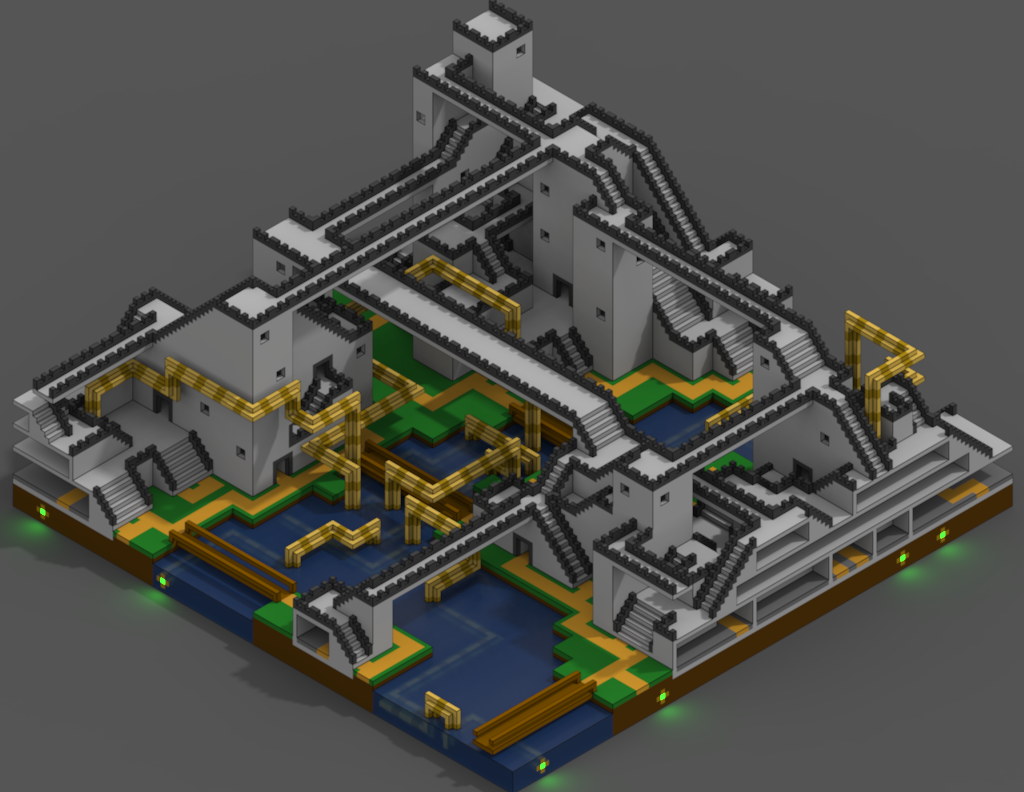
\includegraphics[width=\textwidth]{wfc}
		\end{column}
		\begin{column}{0.55\textwidth}
			\begin{itemize}
                \pause\item Places tiles (2D or 3D) based on constraints on which tiles can be adjacent
                \pause\item An example of \textbf{constraint solving} (similar to e.g.\ solving Sudoku)
			\end{itemize}
		\end{column}
	\end{columns}
\end{frame}

\begin{frame}{$n$-gram models}
	\begin{columns}
		\begin{column}{0.4\textwidth}
			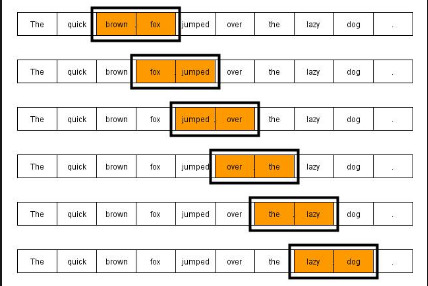
\includegraphics[width=\textwidth]{ngram}
		\end{column}
		\begin{column}{0.55\textwidth}
			\begin{itemize}
                \pause\item Gather frequency data for sequences of length $n$ in some training data
                \pause\item A basic form of machine learning
                \pause\item E.g.\ can train on letters to generate names
                \pause\item E.g.\ can train on words to generate (nonsense) text
                \pause\item E.g.\ can train on tiles to generate levels
			\end{itemize}
		\end{column}
	\end{columns}
\end{frame}



%\part{The role of PCG in games}
\frame{\partpage}

\begin{frame}{Lessons from No Man's Sky}
	\begin{center}
		\pause
\includegraphics[width=0.5\textwidth]{nomanssky_steamreviews}
	\end{center}
	\begin{itemize}
		\pause\item If you overscope, pray that you don't have to cut any features
			that you announced on stage at E3...
		\pause\item PCG is not a substitute for gameplay
		\pause\item PCG is not magic --- it doesn't (by itself) let an indie-sized team produce a AAA game
		\pause\item When talking about scale and PCG, it's easy to set unrealistic expectations
	\end{itemize}	
\end{frame}

\begin{frame}{Big numbers}
	\begin{itemize}
		\pause\item ``Over 18 quintillion planets''
		\pause\item $2^{64} = 18\,446\,744\,073\,709\,551\,616$
		\pause\item What does this number even \textbf{mean}?
		\pause\item What it \textbf{really} means: ``our random number generator uses a 64-bit seed''
		\pause\item They could have said ``a near infinite number of planets''
		\pause\item They could easily have made it ``over 340 undecillion'' planets
			($2^{128} = 340\,282\,366\,920\,938\,463\,463\,374\,607\,431\,768\,211\,456$)
	\end{itemize}
\end{frame}

\begin{frame}{Even bigger numbers}
	\begin{itemize}
		\pause\item There are
			\begin{align*}
		 		52! = 80\,658\,175\,170\,943\,878\,571\,660\,636\,856\,403\,766 &\\
		 		          975\,289\,505\,440\,883\,277\,824\,000\,000\,000\,000 &
		 	\end{align*}
			ways of shuffling a deck of playing cards
		\pause\item When you shuffle a deck, it is almost certain that
			\textbf{no deck of cards in human history} has ever existed in that order
		\pause\item But how \textbf{interesting} is that particular shuffled deck?
		\pause\item How \textbf{different} from another shuffled deck?
	\end{itemize}
\end{frame}

\begin{frame}{Uniqueness}
	``I can easily generate 10,000 bowls of plain oatmeal, with each oat being in a different position 
	and different orientation, and \textit{mathematically speaking} they will all be completely unique.
	But the user will likely just see \textit{a lot of oatmeal}.''
	
	--- Kate Compton
	
	{\tiny\url{http://galaxykate0.tumblr.com/post/139774965871/so-you-want-to-build-a-generator}}
\end{frame}

\begin{frame}{Uniqueness}
	``\thinspace`Every Planet Unique' might mean that each planet has a complex sci-fi backstory rich enough to 
	fill a two-part Star Trek episode.
	It might also mean that, mathematically speaking, there's a rock somewhere on the planet that
	doesn't look like any other rock in the universe.''
	
	--- Michael Cook

	{\tiny\url{http://www.gamesbyangelina.org/2016/08/procedurallanguage/}}
\end{frame}

\begin{frame}{Lessons from Spelunky}
	\begin{center}
		\pause
\includegraphics[width=0.5\textwidth]{spelunky_steamreviews}
	\end{center}
	\begin{itemize}
		\pause\item PCG can complement solid game mechanics
		\pause\item PCG can \textbf{enable} new (discovery-based) game mechanics
		\pause\item No need to dazzle the audience with big numbers
	\end{itemize}	
\end{frame}

\begin{frame}{Curation}
	\begin{columns}
		\begin{column}{0.4\textwidth}
			\pause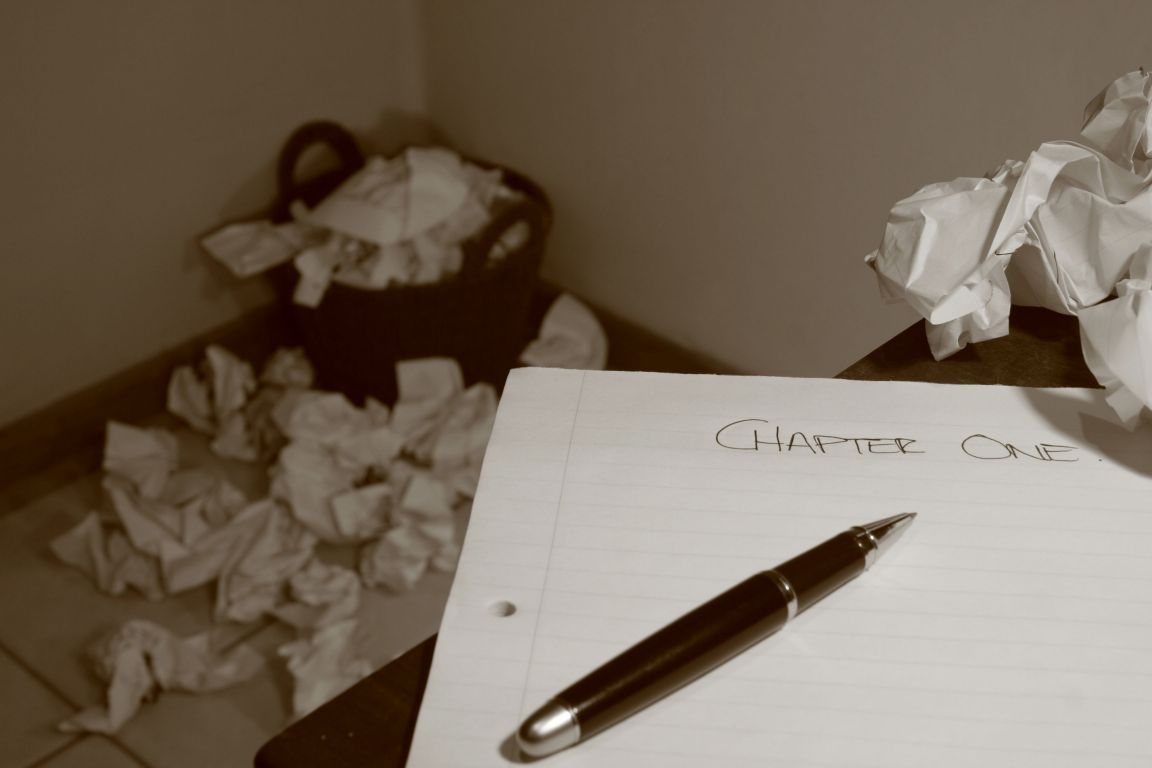
\includegraphics[width=\textwidth]{curation}
		\end{column}
		\begin{column}{0.55\textwidth}
			\begin{itemize}
				\pause\item Human creators constantly ask themselves: \textbf{is this any good?}
				\pause\item Smart PCG should not \textbf{merely generate}: it should also
					\textbf{evaluate}
			\end{itemize}
		\end{column}
	\end{columns}
\end{frame}

\begin{frame}{Authorship}
	\begin{itemize}
		\pause\item In a game with \textbf{emergent narrative}, who is the author?
			Is it the developer, the player, or both?
		\pause\item In a game with \textbf{procedurally-generated content}, who (or what) is the author?
			Is it the developer, the player, the system, or all three?
	\end{itemize}
\end{frame}

\begin{frame}{Authorship}
	``[We] create the systems (including some fixed content), and the choices made at that stage
	are influenced by our preferences, worldviews, talents and flaws, and then the system creates the content.
	The players are exposed to the content and can manipulate it using the tools we (and others) create for them.
	How they use the tools is up to them, and how the content reacts is up to our systems.''
	
	--- Tarn Adams
	
	{\tiny\url{http://www.nullpointer.co.uk/content/interview-dwarf-fortress/}}
\end{frame}



%\part{The future of PCG}
\frame{\partpage}

\begin{frame}
``You are playing an ``open world'' game, something like Grand Theft Auto or Skyrim.
Instead of going straight to the next mission objective in the city you are in,
you decide to drive (or ride) five hours in some randomly chosen direction.
The game makes up the landscape as you go along, and you end up in a new city that no human player has visited before.
In this city, you can enter any house (though you might have to pick a few locks), talk to everyone you meet,
and involve yourself in a completely new set of intrigues and carry out new missions.
If you would have gone in a different direction, you would have reached a different city
with different architecture, different people and different missions.
Or a huge forest with realistic animals and eremites, or a secret research lab, or whatever the game engine comes up with.''

--- Julian Togelius

{\tiny\url{http://togelius.blogspot.co.uk/2015/10/what-if-videogames-had-actual-ai.html}}
\end{frame}

\begin{frame}{Whole game generation}
	\begin{columns}
		\begin{column}{0.4\textwidth}
			\pause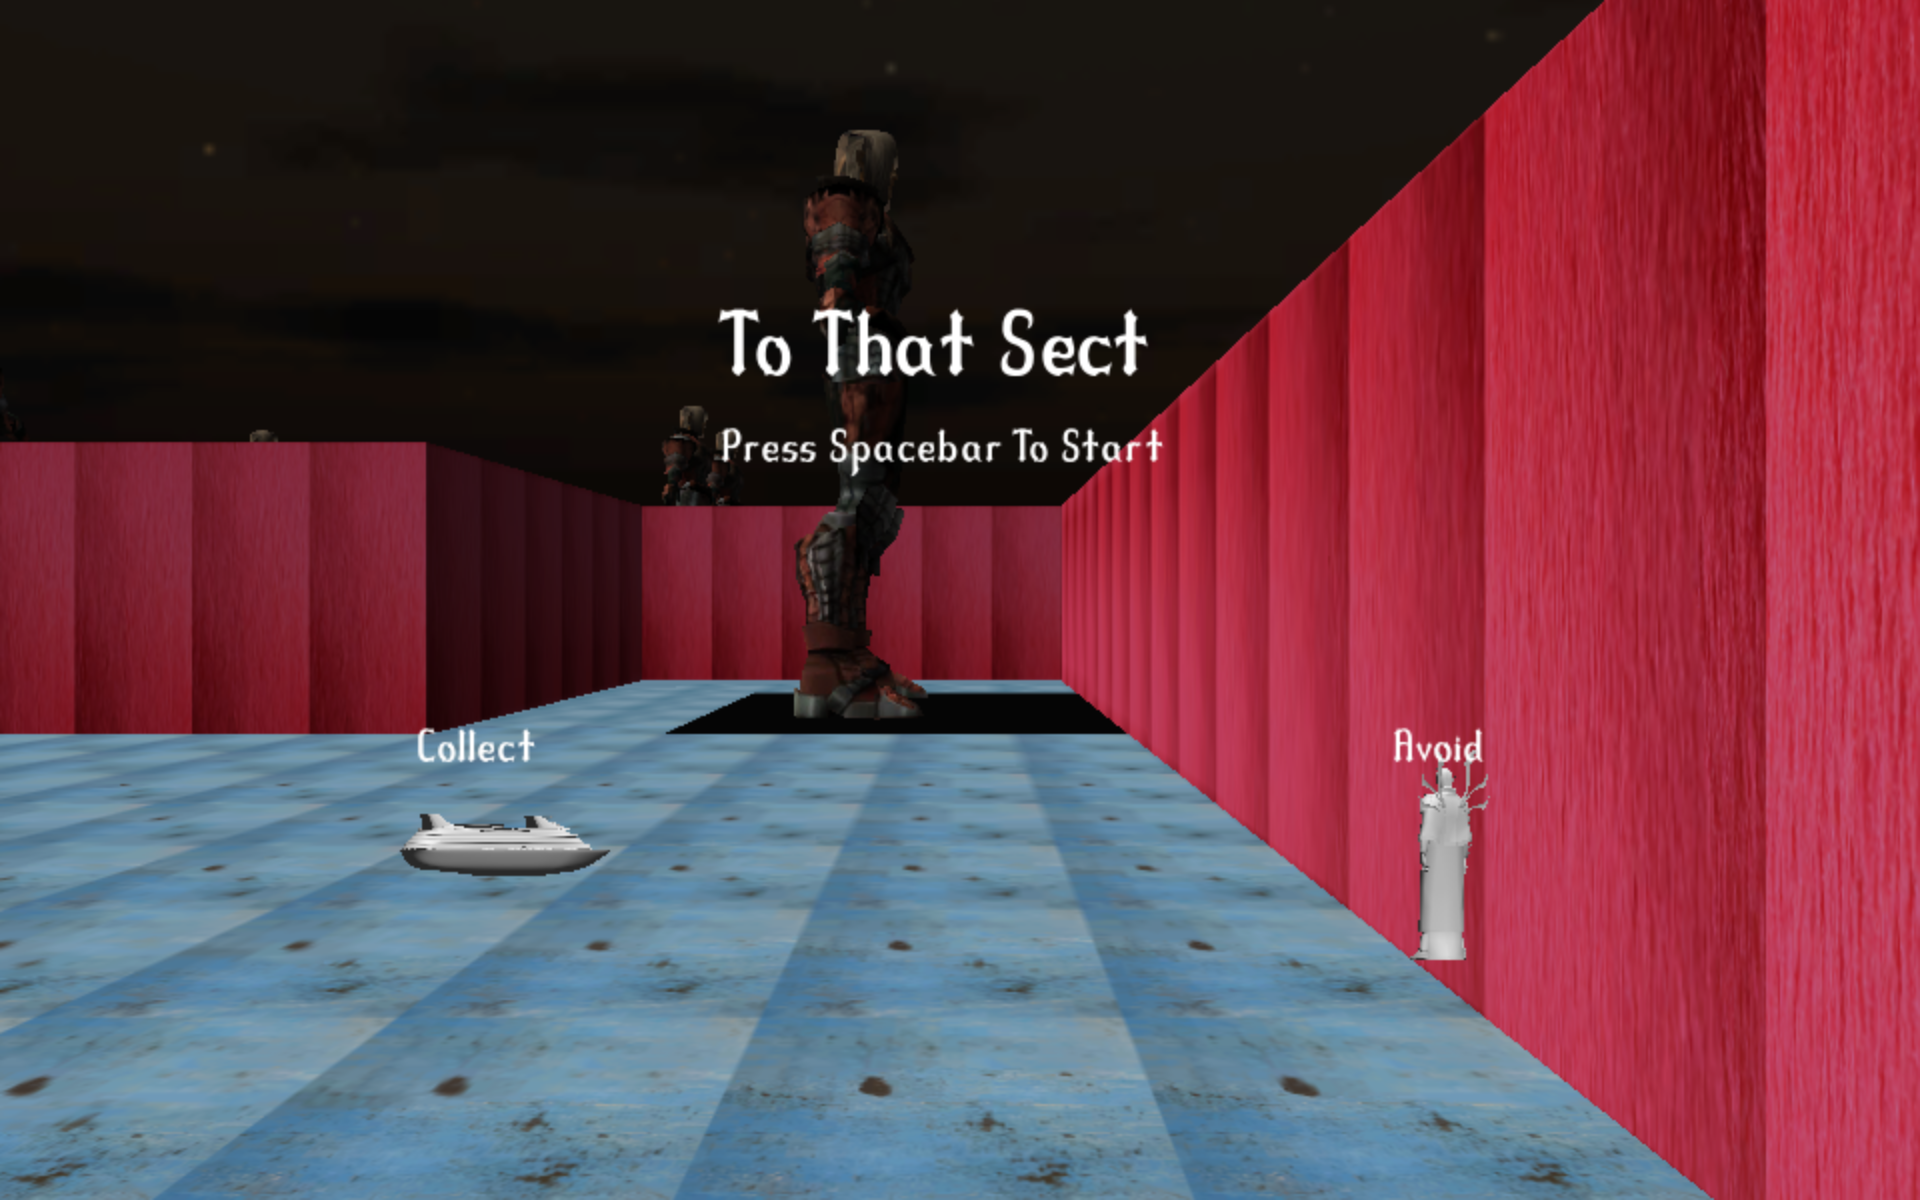
\includegraphics[width=\textwidth]{tothatsect}
		\end{column}
		\begin{column}{0.55\textwidth}
			\begin{itemize}
				\pause\item E.g.\ ANGELINA (Michael Cook)
				\pause\item Generate \textbf{entire games} from scratch, possibly using ideas or themes provided by the user
				\pause\item \textbf{Democratise} game design --- create games in \textbf{collaboration} with a
					non-skilled user
					\begin{itemize}
						\pause\item (i.e.\ make it so that you don't need to do a degree to learn how to make games...)
					\end{itemize}
			\end{itemize}
		\end{column}
	\end{columns}
\end{frame}

\begin{frame}{Computational creativity}
	\begin{columns}
		\begin{column}{0.4\textwidth}
			\pause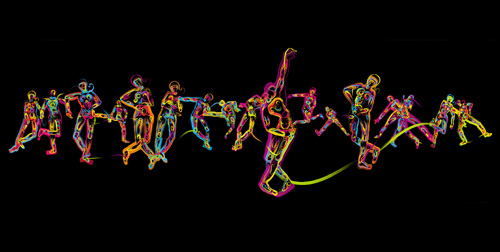
\includegraphics[width=\textwidth]{paintingfool}
			
			\vspace{2ex}
			
			\pause
\includegraphics[width=\textwidth]{beyondthefence}
		\end{column}
		\begin{column}{0.55\textwidth}
			\begin{itemize}
				\pause\item Open question: can an AI system be \textbf{creative}?
				\pause\item Beyond \textbf{mere generation}
				\pause\item Beyond generating \textbf{content} to generating \textbf{ideas}
			\end{itemize}
		\end{column}
	\end{columns}
\end{frame}


\end{document}
